%!TEX root = ../thesis.tex
% ******************************* Thesis Appendix B ********************************

\chapter{Data Structure}






\begin{table}[]
\centering
\caption{}
\label{tab:my-table}
\begin{tabular}{lc}
\hline
attribute                                   & description                             \\ \hline
Forname                                     & anonymised                              \\
Surname                                     & anonymised                              \\
DOB                                         & dd/mm/yyyy partially anonymised to year \\
Sex                                         & boolean                                 \\
Medical\_Card                               & structured                              \\
ID\_Case\_Entry\_Date                       & date-time                               \\
Case\_No                                    & integer                                 \\
Appointment\_Time                           & inoperative/unreliable                  \\
Relationship\_to\_Caller                    & unstructured                            \\
PriorityOnReception                         & structured                              \\
PriorityAfterAssessment                     & structured                              \\
Cons\_Start\_Date                           &                                         \\
Cons\_End\_Date                             &                                         \\
Consult\_Type                               & structured                              \\
Cons\_Time\_Taken                           &                \\
Consult\_Type                               & structured                              \\

\textbf{OLC\_History}      & free-text                                         \\
\textbf{OLC\_Examination}  & free-text                                         \\
\textbf{OLC\_Diagnosis}    & free-text                                         \\
\textbf{OLC\_Treatment}    & free-text                                         \\
\textbf{Teleguides\_Notes} & free-text                                        
\end{tabular}
\end{table}


\begin{figure}[!t]
\centering
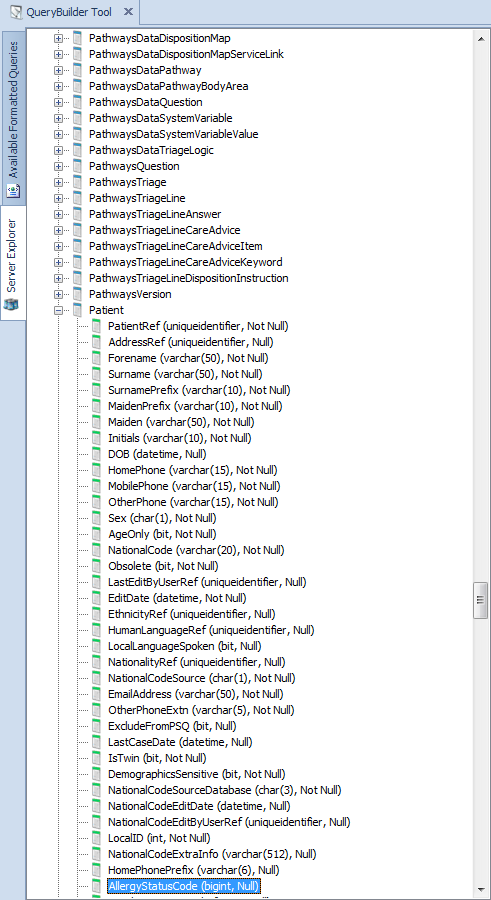
\includegraphics[width=4.0in]{Figs/table-caredoc.png}
% where an .eps filename suffix will be assumed under latex, 
%% and a .pdf suffix will be assumed for pdflatex; or what has been declared
 \DeclareGraphicsExtensions.
\caption{Sample view of Caredoc internal database}
\label{fig:internal-caredoc}
\end{figure}